\part{Features}

\chapter{Backend API}

\section{Ready}

Here is a list of the routes already availables from the backend API. All the routes below are preceded by \url{http://ip_server:port/api}

\subsection{Global}
\begin{itemize}
	\item GET "/"
	\begin{itemize}
		\item Returns "Hello World"
	\end{itemize}
\end{itemize}

\subsection{Users}
\begin{itemize}
	\item POST "/users"
	\begin{itemize}
		\item Create a user
	\end{itemize}
\end{itemize}

\begin{itemize}
	\item POST "/auth"
	\begin{itemize}
		\item Authenticate a user
	\end{itemize}
\end{itemize}

\begin{itemize}
	\item GET "/users"
	\begin{itemize}
		\item This route send back every public informations about every users. It can be a bit heavy with a lot of users.
	\end{itemize}
\end{itemize}

\begin{itemize}
	\item GET "/users/:usrid"
	\begin{itemize}
		\item This route send back the public informations about the chosen user
	\end{itemize}
\end{itemize}


\begin{itemize}
	\item PUT "/users/:usrid"
	\begin{itemize}
		\item This route update the information about the chosen user.
	\end{itemize}
\end{itemize}


\begin{itemize}
	\item DELETE "/users/:usrid"
	\begin{itemize}
		\item This route deletes the chosen user.
	\end{itemize}
\end{itemize}

\subsection{Routes}
\begin{itemize}
	\item GET "/routes"
	\begin{itemize}
		\item This route send back every informations about all the routes. It can be a bit heavy with a lot of routes.
	\end{itemize}
\end{itemize}


\begin{itemize}
	\item GET "/routes/:routeid"
	\begin{itemize}
		\item This route send back the public informations about the chosen route.
	\end{itemize}
\end{itemize}


\begin{itemize}
	\item GET "driverroutes/:driverid"
	\begin{itemize}
		\item This route send back the public informations about all the routes from a specific driver.
	\end{itemize}
\end{itemize}

\begin{itemize}
	\item GET "driverroutesdate/:driverid"
	\begin{itemize}
		\item To get the route where the user's id is the driver order by date.
	\end{itemize}
\end{itemize}

\begin{itemize}
	\item PUT "/routes"
	\begin{itemize}
		\item This route create a new Route in the database. It search the optimal directions with the google maps API, in order to store the best route.
	\end{itemize}
\end{itemize}

\begin{itemize}
	\item DELETE "/routes/:routeid"
	\begin{itemize}
		\item This route deletes the chosen route.
	\end{itemize}
\end{itemize}

\begin{itemize}
	\item POST "/routes/findTarget"
	\begin{itemize}
		\item 	This route can be used in order to search for a route that match specific parameters.
	\end{itemize}
\end{itemize}

\subsection{Route Dates}
\begin{itemize}
	\item GET "/routedate/:routeid"
	\begin{itemize}
		\item This route send back the public informations about the chosen routedate.
	\end{itemize}
\end{itemize}

\begin{itemize}
	\item GET "/routedate"
	\begin{itemize}
		\item This route returns all the routedates for all the routes.
	\end{itemize}
\end{itemize}

\subsection{Rides}
\begin{itemize}
	\item GET "/rides"
	\begin{itemize}
		\item This route send back every informations about all the rides. It can be a bit heavy with a lot of rides.
	\end{itemize}
\end{itemize}

\begin{itemize}
	\item GET "/rides/:rideid"
	\begin{itemize}
		\item This route send back the public informations about the chosen ride.
	\end{itemize}
\end{itemize}

\begin{itemize}
	\item GET "/rides/route/:passengerId"
	\begin{itemize}
		\item This route show all the routes that the passenger add to his rides.
	\end{itemize}
\end{itemize}

\begin{itemize}
	\item GET "/rides/routeId/:routeId"
	\begin{itemize}
		\item This route show the ride id corresponding to this route id.
	\end{itemize}
\end{itemize}

\begin{itemize}
	\item POST "/rides"
	\begin{itemize}
		\item This route create a ride in the database.
	\end{itemize}
\end{itemize}

\begin{itemize}
	\item PUT "/rides/:rideid"
	\begin{itemize}
		\item This route update the information about the chosen ride.
	\end{itemize}
\end{itemize}

\begin{itemize}
	\item  DELETE "/rides/:rideid"
	\begin{itemize}
		\item This route deletes the chosen ride.
	\end{itemize}
\end{itemize}

\subsection{Passenger}
\begin{itemize}
	\item GET "/passengers"
	\begin{itemize}
		\item This route send back every informations about all the passengers. It can be a bit heavy with a lot of passengers.
	\end{itemize}
\end{itemize}

\begin{itemize}
	\item GET "/passengers/:passid"
	\begin{itemize}
		\item This route send back the public informations about the chosen passenger.

	\end{itemize}
\end{itemize}

\begin{itemize}
	\item GET "/passengers/route/:passId"
	\begin{itemize}
		\item Query that returns the information of route where the user is a passenger order by date.
	\end{itemize}
\end{itemize}

\begin{itemize}
	\item GET "/passengers/information/:routeId"
	\begin{itemize}
		\item Query that returns the information of passengers who are using the ride.
	\end{itemize}
\end{itemize}

\begin{itemize}
	\item POST "/passenger"
	\begin{itemize}
		\item 	This route can create a passenger in the database.
	\end{itemize}
\end{itemize}

\begin{itemize}
	\item POST "/passenger/existingRide"
	\begin{itemize}
		\item 	This route create a passenger for a already existing Ride where the id of the route is in parameter with the id of the passenger.
	\end{itemize}
\end{itemize}

\begin{itemize}
	\item PUT "/passenger/:passid"
	\begin{itemize}
		\item This route update the information about the chosen passenger.
	\end{itemize}
\end{itemize}

\begin{itemize}
	\item DELTE "/passenger/:passid"
	\begin{itemize}
		\item This route deletes the chosen passenger.
	\end{itemize}
\end{itemize}

\begin{itemize}
	\item GET "/passenger/alert/:driverId"
	\begin{itemize}
		\item Query that returns the name of all passengers in relation to a driver (For the alert message at startup)
	\end{itemize}
\end{itemize}

\begin{itemize}
	\item POST "/passenger/alert/:driverId"
	\begin{itemize}
		\item This route create a passenger for a already existing Ride where the id of the route is in parameter with the id of the passenger
	\end{itemize}
\end{itemize}

\begin{itemize}
	\item PUT "/passenger/alert/:passId"
	\begin{itemize}
		\item This route create a passenger for an un-existing Ride where the id of the route is in parameter with the id of the passenger
	\end{itemize}
\end{itemize}

\subsection{Ratings}
\begin{itemize}
	\item GET "/ratings"
	\begin{itemize}
		\item 	This route send back every informations about all the ratings. It can be a bit heavy with a lot of rates.
	\end{itemize}
\end{itemize}

\begin{itemize}
	\item GET "/ratings/:rateid"
	\begin{itemize}
		\item This route send back the public informations about the chosen rate.
	\end{itemize}
\end{itemize}

\begin{itemize}
	\item GET "/ratings/:targetid"
	\begin{itemize}
		\item This route send back the the average of rate concerning the target.
	\end{itemize}
\end{itemize}

\begin{itemize}
	\item POST "/ratings"
	\begin{itemize}
		\item This route create a rate in the database.
	\end{itemize}
\end{itemize}

\begin{itemize}
	\item POST "/ratings/existingRate"
	\begin{itemize}
		\item This route can modify a rate in the database if the rate already exist.
	\end{itemize}
\end{itemize}

\begin{itemize}
	\item DELETE "/ratings/:rateid"
	\begin{itemize}
		\item This route update the information about the chosen rating.
	\end{itemize}
\end{itemize}

\begin{itemize}
	\item GET "/ratings/Comment/:targetid"
	\begin{itemize}
		\item This route send back the comments regarding the chosen target
	\end{itemize}
\end{itemize}

\subsection{Favorite Route}
\begin{itemize}
	\item GET "/favoriteRoute/:userId"
	\begin{itemize}
		\item This routes returns all the favorites routes of a chosen user.
	\end{itemize}
\end{itemize}

\begin{itemize}
	\item POST "/favoriteRoute"
	\begin{itemize}
		\item This route create a favorite route.
	\end{itemize}
\end{itemize}

\begin{itemize}
	\item DELETE "/favoriteRoute"
	\begin{itemize}
		\item This route delete a favorite route.
	\end{itemize}
\end{itemize}

\section{To Do}

Currently, there is no need to add additional features to the backend API.

\chapter{Android application}

\section{Ready}
\begin{itemize}
	\item {\bf Page 1 : Login}. This page is fully working. The user can log in or register by clicking on the "Sign in" button.
	\item {\bf Page 2 : Sign in}. This page is fully working. The user can register by filling the form and pressing the button "Create an account".
	\item {\bf Page 3 : Home}. The map is displayed on the background. Also, we can search for a ride, or navigate trough the navbar.
	\item {\bf Page 4 : Navbar}. The navbar is fully working. The user can access to his profile, his lifts, page help, settings and logout.
	\item {\bf Page 5 : Lift}. This page is working. The search is working also. The user can select his origin, his destination, and the date where he want to travel.
	\item {\bf Page 6 : Availables drives}. This page is fully working. You can click on a available ride to display it in the page 7. You can also click on "I want to drive" to create your own ride.
	\item {\bf Page 7 : User x's route}. This page is fully working. You can see the driver's route, and also the path between your starting point and the meeting point with the driver. Idem for the your ending point and the dropping point.
	\item {\bf Page 9 : User profile}. This page is working. You access to the user's details, including first and last name, username, rating, and mobile number.

\item {\bf Page 3 : Home}. The map is not focused on the user's location.
\item {\bf Page 5 : Lift}. There is no button to enter the current location of the user in the origin field. Also, the management of the weekly recurrence is not implemented.
	\item {\bf Page 8 : Create your route}. This page is not implemented currently.
	\item {\bf Page 9 : User profile}. Clicking on the user's number should start a call on the phone.
	 \item {\bf Page 10 : My drives}. This page is not implemented currently.
	 \item {\bf Page 11 : Help}. This page is not implemented currently.
	 \item {\bf Page 12 : Settings}. This page is not implemented currently.
\end{itemize}

\newpage
\section{Login and Sign in}
Class : LoginActivity and SignInActivity \\
Description :  The user can log in or register by clicking on the create an account button and fillout the form.\newline

\begin{figure}[h!]
   \begin{minipage}[b]{0.48\linewidth}
      \centering 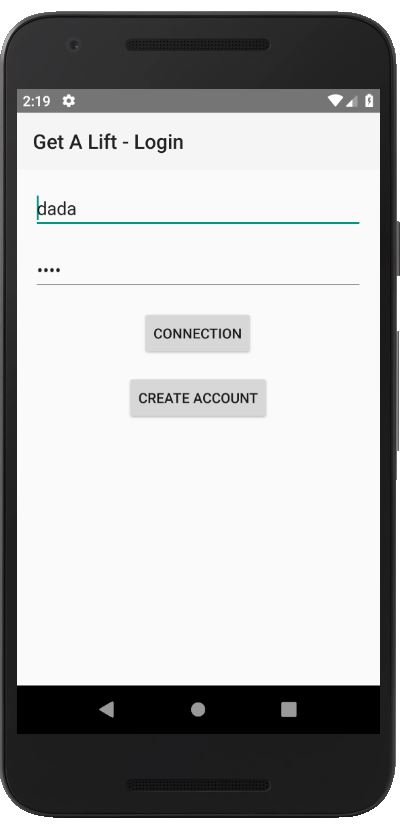
\includegraphics[scale = 0.8]{diagrams/login_page.jpg}
\caption{\it Login Page}
   \end{minipage}\hfill
   \begin{minipage}[b]{0.50\linewidth}   
      \centering 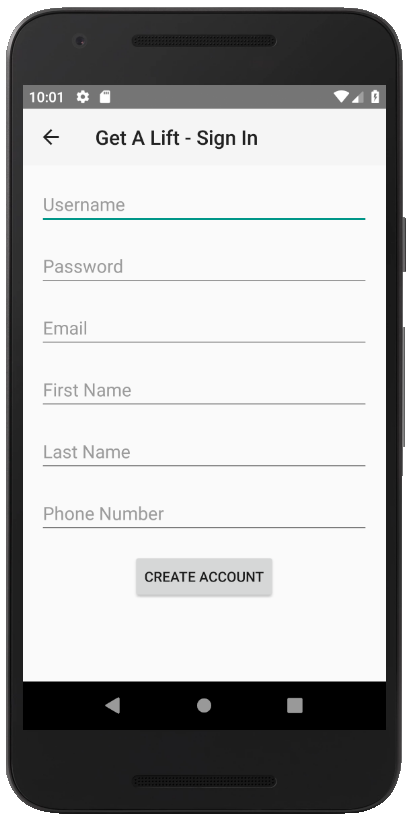
\includegraphics[scale = 0.8]{diagrams/Create_account.png}
      \caption{\it Sign in Page}
   \end{minipage}
\end{figure}

\section{Home and NavBar}
Class : HomeMapActivity \\
Description : The map is displayed on the background. Also, we can search for a ride, or navigate trough the navbar. The user can access to his prfile, his lifts, page help, settings and logout. \\
More details : The map show the last position registered by the phone but if this data is null (as on the emulator at the beginning), it will show the University of Malta. 

\begin{figure}[h!]
\begin{center}
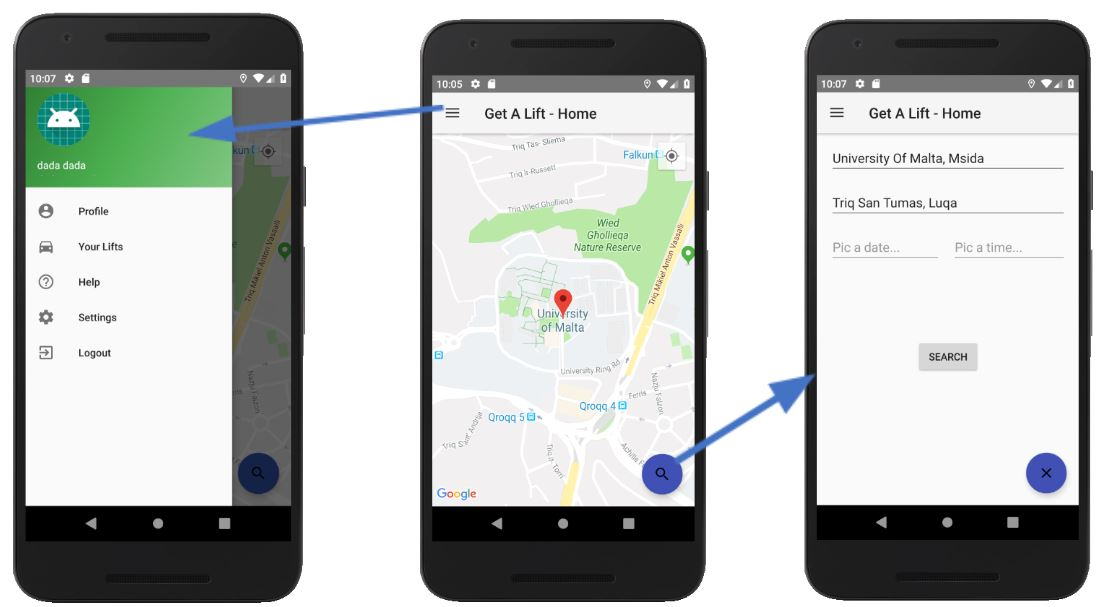
\includegraphics[scale = 0.6]{diagrams/HomePage_gal.JPG} 
\end{center}
\end{figure}

\section{Available drives}
Class : ResultSearchActivity \\
Description : You can click on a available ride to display it. You can also click on "I want to drive" to create your own ride. \\
Bugs : It shows all the drives corresponding to the research even that one who did pass and where the user is driver.

\begin{figure}[h!]
\begin{center}
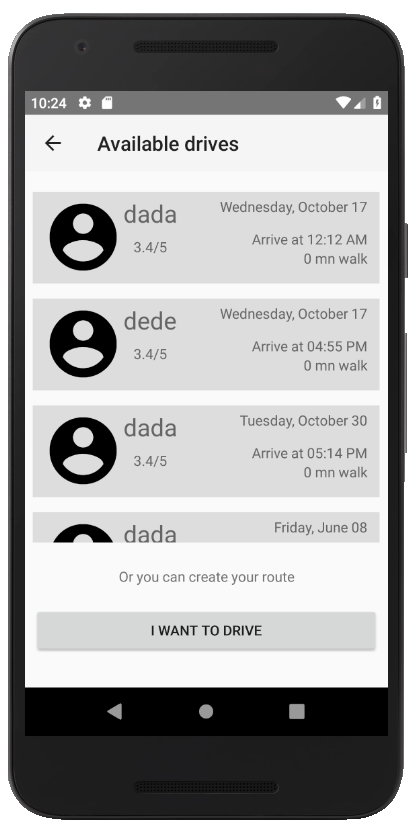
\includegraphics[scale = 0.6]{diagrams/Available_drives.png} 
\end{center}
\end{figure}

\section{User's x's route}
Class : ViewRideActivity \\
Description : You can see the driver’s route, and also the path between your starting point and the meeting point with the driver. Idem for the ending point and the dropping point. When the user clicks on “Go!”, he is redirected to a page with all the info about the route and the driver.

\begin{figure}[h!]
\begin{center}
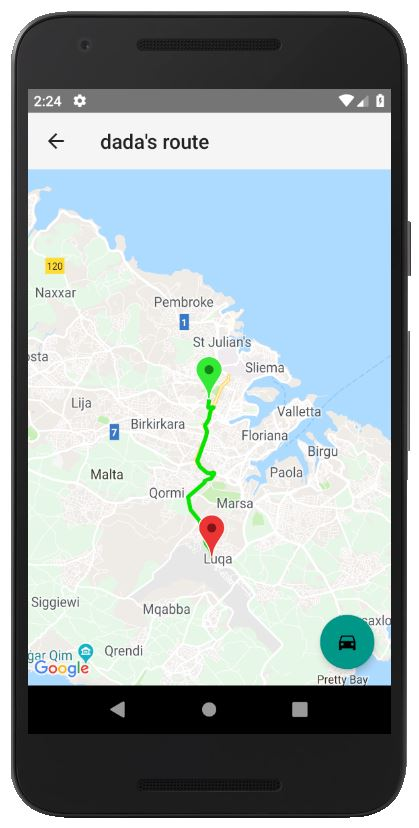
\includegraphics[scale = 0.6]{diagrams/ViewRide_page.jpg} 
\end{center}
\end{figure}

\section{User's x's route info}

Class : ViewRideInfoActivity\\
Description : The user can see the driver’s route information, and confirm that he wants to be passenger on this ride.  The use can also call the driver and send him a message by clicking on the icons\\
After this confirmation, the app check if the route is already added to the ride in the database. If not, it adds it. After, the app checks if the user is already a passenger in this ride and send a notification to the driver if it’s not the case.
\newline
Id the user is already driver, a notification appear also.\\
Better : Before display the availables drives, sort out to not display the drives where the user is driver. 
\begin{figure}[H]
\begin{center}
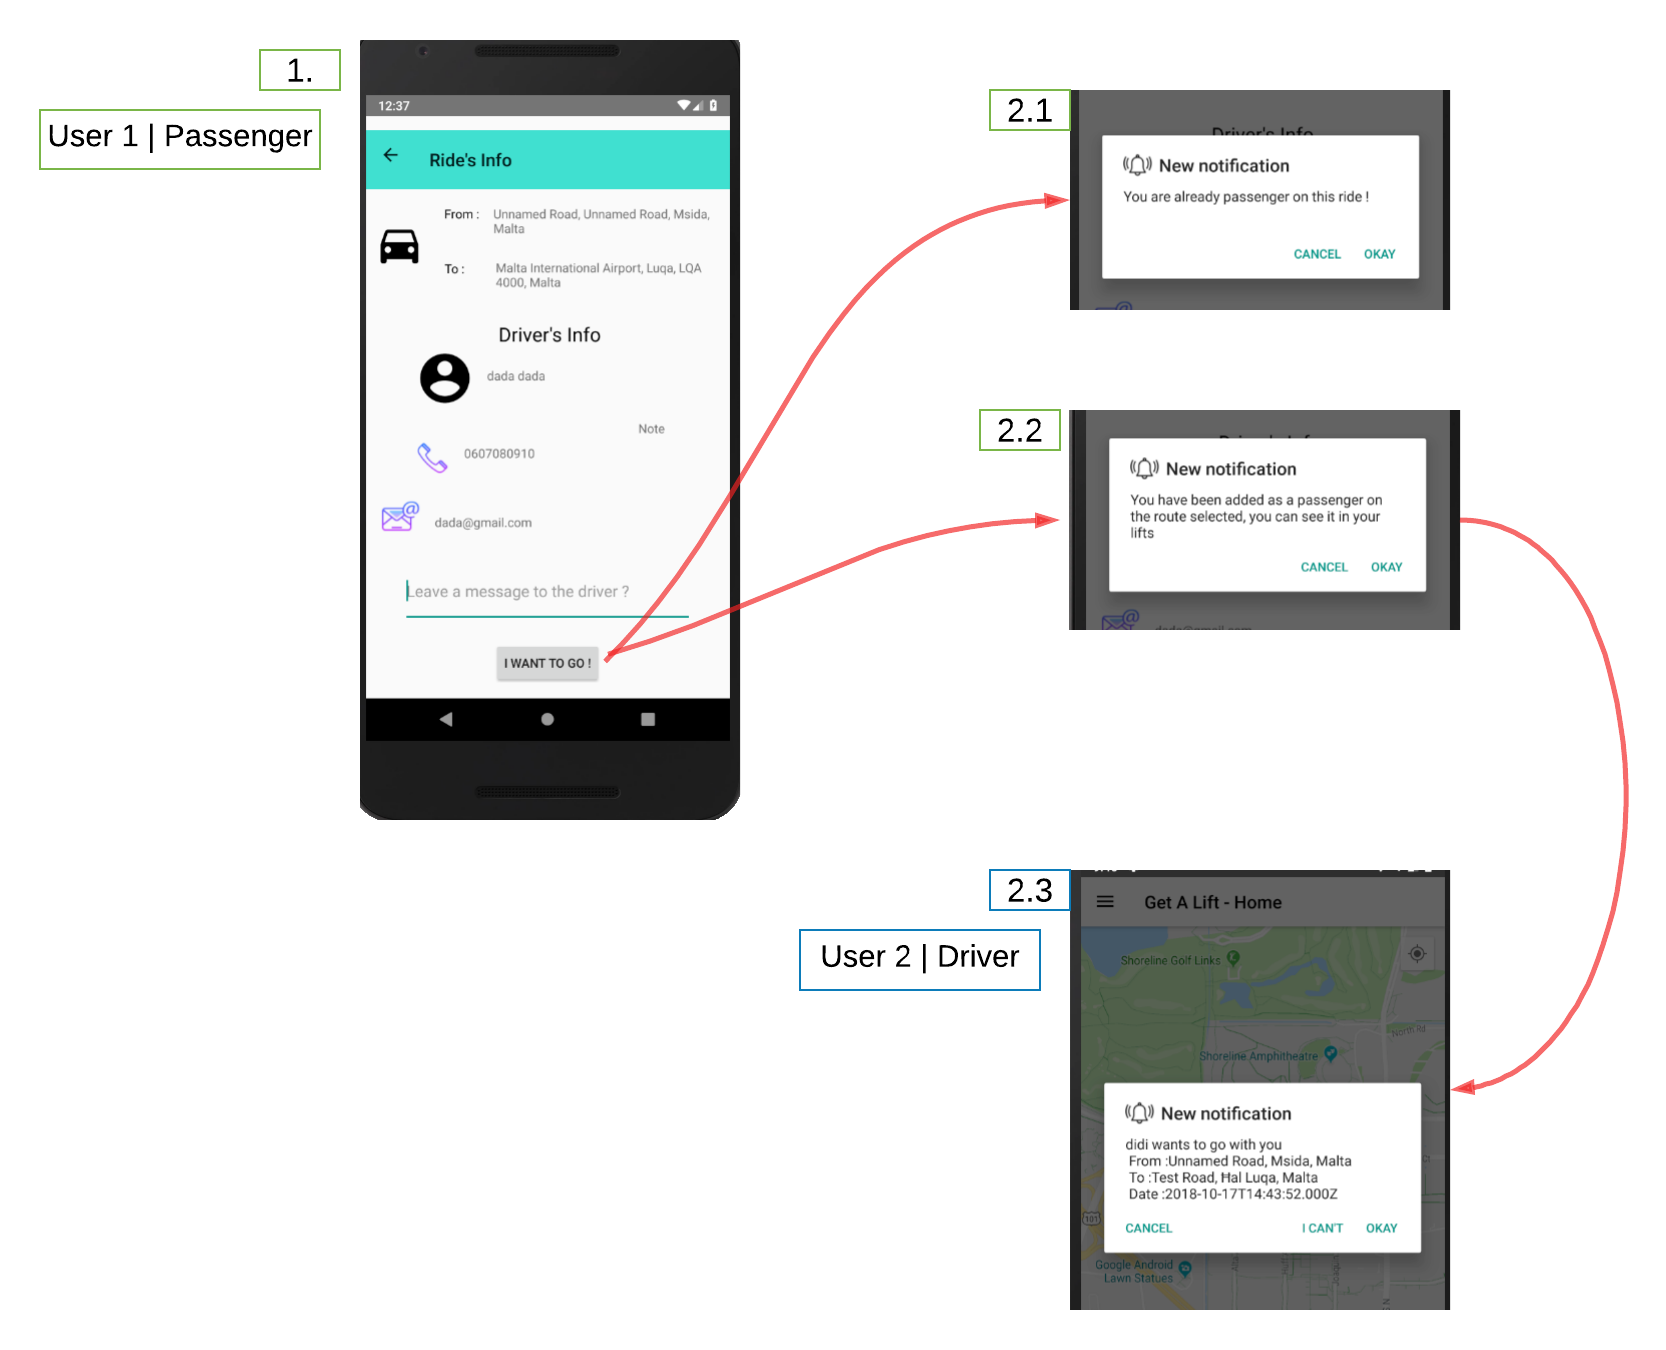
\includegraphics[scale = 0.3]{diagrams/maquette_notif_pass-dri.png} 
\end{center}
\end{figure}

TO DO :
\begin{enumerate}
\item[•] Replace alerts by notification to see them outside the app
\item[•] Advert the passenger if the driver say 'no'
\item[•] Improve the design (like IOS version)
\end{enumerate}

\section{User's profile}
Class : ProfileActivity \\
Description : You access to the user’s details, includingfirst and last name, username, rating, and mobile number..\\
Here, we recover the information of teh current user thanks to "SharedPreference". This information is stored when the user connect himself.

\begin{figure}[H]
\begin{center}
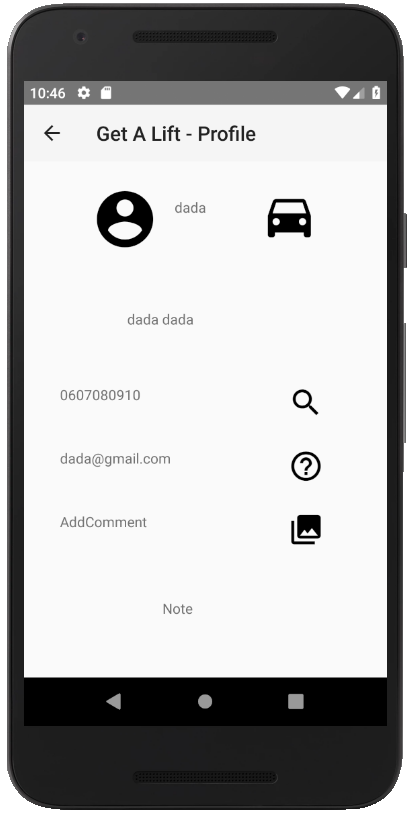
\includegraphics[scale = 0.6]{diagrams/Profile.png} 
\end{center}
\end{figure}

\section{Create a route}
\textbf{Class :} CreateRideActivity, CreateRideInfoActivity, DirectionJSONParser \newline

\textbf{Description :} Allow the user to create a route directly on a Google Map. \newline

\textbf{More details : }First, he can see two markers placed in function of his precedently research linked by an itinerary. And in the same time, a message is displayed to inform the user that he can edit the route by dragging the two markers on the map.\\ After that, he can confirm by clicking on the green button.Thus, he is redirected on the Created route’s info and there, he will confirm. \newline

In this page, he can see all the details on the route created and add the date and the time. He can also go back edit the new route by clicking on the edit button (at the bottom on the left) and will return on the page with his new route created.
So the back button on the toolbar redirects him to the home page. \\ 
The picture is in French but the functionality has been made in English too.

\begin{figure}[H]
\begin{center}
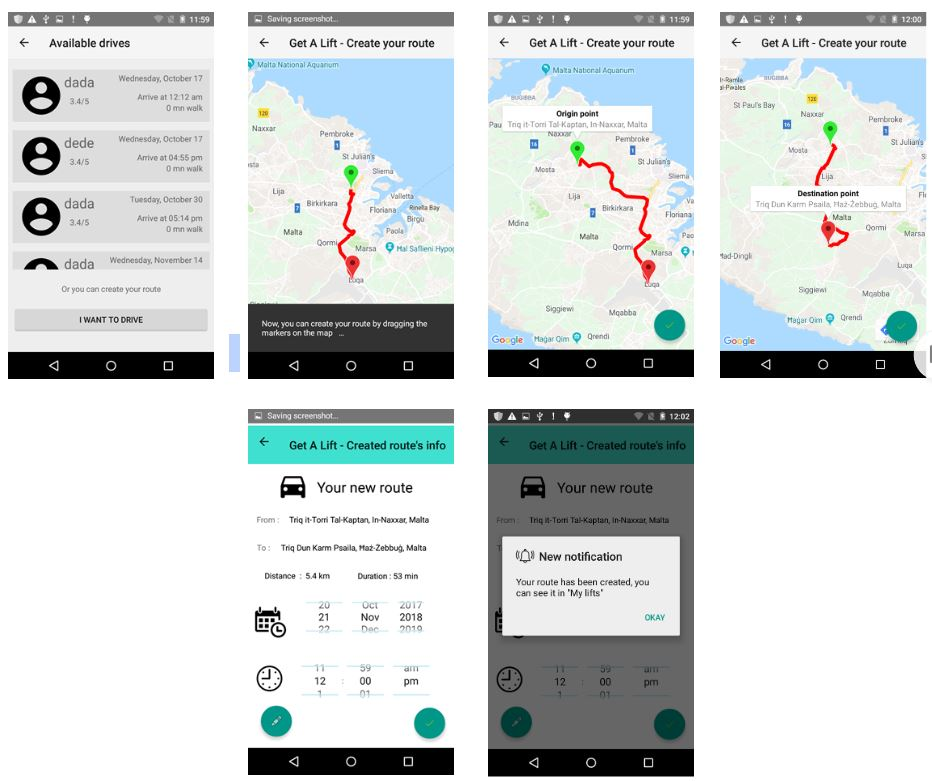
\includegraphics[scale = 0.9]{diagrams/Create_route.JPG} 
\end{center}
\end{figure}

There, I found the code (to draw a line between two marker by clicking on the map) in Internet and I adapted it (to be able to drag the markers, update the itinerary and display the new adresse after dragging) : to display the itinerary by Google API Direction. \newline
The class DirectionsJSONParser is to use the response given by google : \\
 \url{https://maps.googleapis.com/maps/api/directions/json?origin=University+of+Malta&destination=196+Triq+Leli+Falzon&key=AIzaSXXXXXXXXXXXX} \\
(You can try it on a web navigator to see) by replacing AIzaSXXXXXXXXXXX by a valid Google API Key associated with a billing account (new Google rule for his API access since 11 June 2018). \newline
\textbf{I WILL DELETE MY API KEY, YOU HAVE TO CREATE  NEW ONE WITH A BILLING ACCOUNT TO SEE THE FUNCTIONALITIES LINKED TO GOOGLE METHODS.}


\section{User's Drives}


\textbf{Classes : } DriveActivity, DriveAdapter, DriveList, PassengerList, DriveDetails, Drive \newline

\textbf{Description : } You access to the user’s drive, all the drive which are link to the user (When he is the driver and when he is the passenger) including  the Origins Address, the Destination Address and the Date of the drive. \\ The page is divided into 2 lists (1 as a Driver and 1 as a Passenger). When you click on a drive, you got information on that Drive including the origins, the destination, the duration, the name of the driver and the list of passenger. You can also get information on the driver or the passenger when you click on their name, their profile page open.

\begin{figure}[H]
\begin{center}
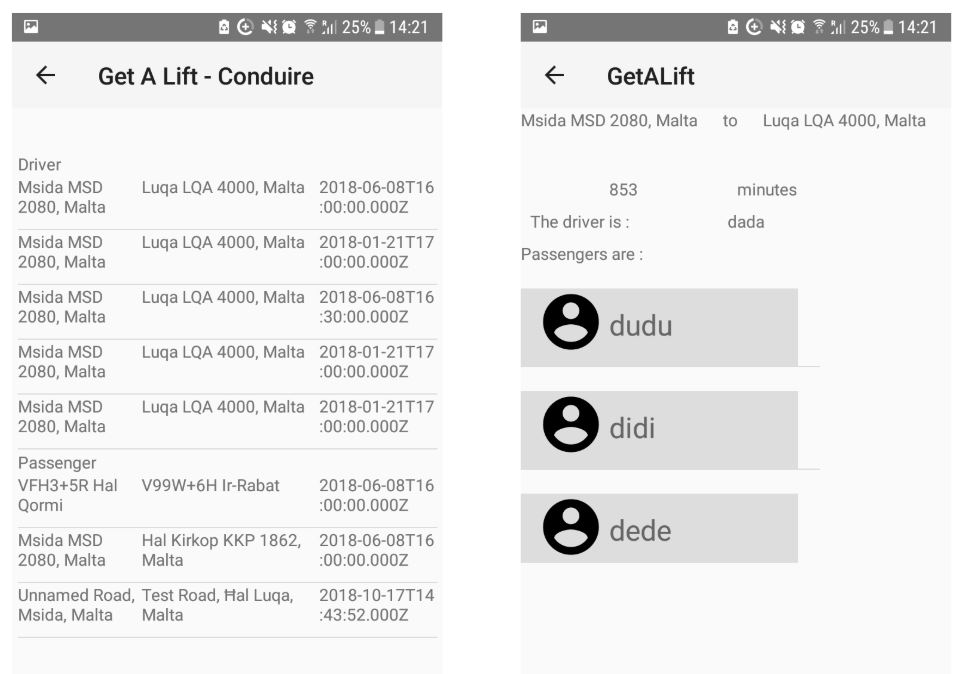
\includegraphics[scale = 0.7]{diagrams/Drive_page.JPG} 
\end{center}
\end{figure}

Bugs : the date format on the lists of drive. We think that it’s due to jet lag.\\
TO DO :  Manage this problem and improve the design

\section{Rating system}

Class : RatingSystem \newline
Description : Allow the user to rate other user with a rate (between 0 and 5) and a comment. To access at this page, we need to see the user’s profile that we want rate from the drive details list.  \newline
For rating someone, there are 2 steps : 
\begin{enumerate}
\item[•]First you choose a rate and write a comment (not required) and you click on the commit button. 
\item[•] Then a message appears to show you what you have selected and asks you for confirmation, so you need to click on another button which will appears.\\ 

To know if you can rate the user or no, a boolean is send form the Drive List into the profile page to block you if you can’t rate the user. (You can’t rate a user when you share no drive with him or when you are on your own profile)

\end{enumerate}

\begin{figure}[H]
\begin{center}
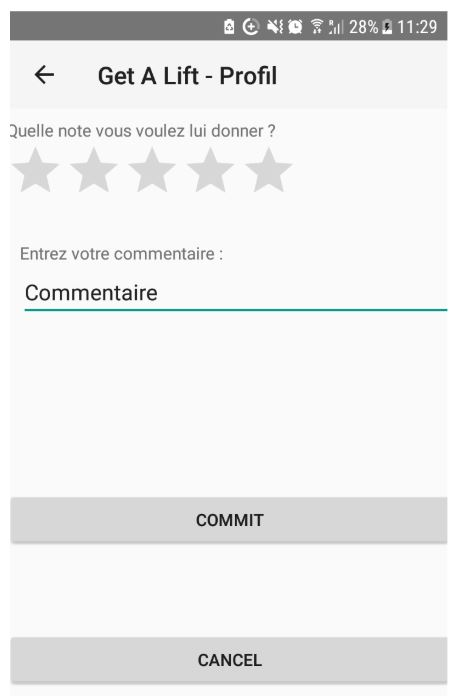
\includegraphics[scale = 0.7]{diagrams/rating_page.JPG} 
\end{center}
\end{figure}
TO DO : \\
\begin{enumerate}
\item[•] A function that return the good format of the date.
\item[•] Prevent a user to rate himself 
\item[•] A way to prevent the user to modify the rate when he is in the Validation mode 
\item[•] A new page that allow the user to see the comment of the user that he select
\end{enumerate} 


